\documentclass[a4paper,fleqn,11pt]{article}

\usepackage[margin=25mm]{geometry}

\listfiles
\newcommand{\bx}[1]{\fbox{\begin{minipage}{12cm}#1\end{minipage}}}
\usepackage{url,apalike,amsmath}
\usepackage[pdftex]{graphicx}
\usepackage[small]{titlesec}
\usepackage{gensymb}
\usepackage{color}

\begin{document}

\large\noindent\textbf{Searching for Unknotting Sequences using
  Machine Learning}\\
\\
%% authorlist
\normalsize

\medskip
\hrule
\medskip

%%%%%%%%%%%%%%%%%%%%%%%%%%%%%%%%%%%%%%%%%%%%%%%%%%%%%%%%%%%%%%%%%%%%%%%%%%
\section{Introduction}

\bx{motivation - why are we doing this? Perhaps contextualise this in
  the idea of different kinds of computational tools for mathematics
  research: we are accustomed to tools that }

%%%%%%%%%%%%%%%%%%%%%%%%%%%%%%%%%%%%%%%%%%%%%%%%%%%%%%%%%%%%%%%%%%%%%%%%%%
\section{Problem Description}

The problem that the program is solving is as follows: given a knot
and a set of operators that can make changes to that knot, find a
sequence of operators that, when applied sequentially to the knot,
result in the unknot.

\bx{describe problem in detail. give details of what each of the
  operators does}

%%%%%%%%%%%%%%%%%%%%%%%%%%%%%%%%%%%%%
\subsection{Notation}

In order to carry out computations on knots, a notation is needed that
can be manipulated by the algorithm. In this work we use an augmented
version of the Dowker-Thistlethwaite code~\cite{DT83}---call this
\emph{aDT}. For a knot with $n$ crossings, their paper describes a
method which assigns a pair of positive integers from $[1,2n]$ to each
crossing, by the following process. Given a knot diagram, give the knot
strand a direction, and assign a starting point on a strand. Follow
the strand in that direction, and each time a crossing is encountered,
assign the lowest number from $[1,2n]$ that has not previously been
used. This process assigns an even/odd pair to each crossing. The
pairs can therefore be listed in numerical order by the odd crossing,
and the knot represented by an ordered list $[c-1,\ldots,c_n]$ of the
corresponding even crossings. This is then annotated further by adding
a positive or negative sign to indicate which strand is the
over-strand: $c_i$ is positive if the over-strand corresponds to the odd
number, and negative in the other case. Call this the \emph{basic DT code}.

However, there is an a ambiguity in this notation. Consider the knot
in figure~\ref{fi:ambiguous}. The same basic DT code encodes for both
of the knot diagrams in the figure. This ambiguity can be resolved by
adding to the code an ordered list of length $n$ of $+1$s and
$-1$s---call this the \emph{orientation} of the crossing. In this list
+1 means that the oriented over-strand, when rotated counter-clockwise
by $90\degree$ aligns with the oriented under-strand (regardless of
the odd or even labeling), and -1 in the other case
(Figure~\ref{fi:orientation}).

\begin{figure}
  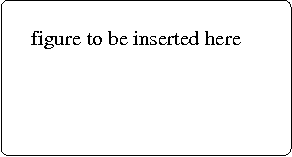
\includegraphics[width=90mm]{blank.png}
  \caption{Example of a knot where the basic DT code does not provide
    enough information to distinguish between two
    diagrams. \textcolor{red}{(Do I mean ``diagrams'' here?)}.}
  \label{fi:ambiguous}
\end{figure}

\begin{figure}
  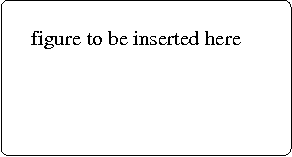
\includegraphics[width=90mm]{blank.png}
  \caption{Description of the orientation.}
  \label{fi:orientation}
\end{figure}

%%%%%%%%%%%%%%%%%%%%%%%%%%%%%%%%%%%%%
\subsection{Operators}

In order to carry out the unknotting process we define a number of
\emph{operators} that will be used to build the unknotting
sequences. These are:
\begin{itemize}\addtolength{\itemsep}{-0.5\baselineskip}
  \item \emph{R1up}/\emph{R1down}: the Reidermeister type 1 move; up
    means including a new loop, down means removing a loop.
  \item \emph{R2up}\emph{R2down}: the Reidermeister type 2 moves; up
    means creating two new crossings by pushing a strand under/over
    other one, down means removing two crossings where by pulling a
    strand from under/over another one.
  \item \emph{R3}: the Reidermeister type 3 move.
  \item \emph{CC}: a crossing change from down to up or vice versa.
  \item \emph{Shift:} shifting the labels along the strand by one
    position.
\end{itemize}

%%%%%%%%%%%%%%%%%%%%%%%%%%%%%%%%%%%%%%%%%%%%%%%%%%%%%%%%%%%%%%%%%%%%%%%%%%
\section{Algorithm}

Genetic algorithms (GAs) are a population-based search heuristic,
designed to efficiently search a large space of possible solutions to
a problem. They are inspired by biological evolution, and work
iteratively on a large set of possible solutions, called the
population. At each iteration the best solutions in the population are
selected, pairs of them combined (crossover) and small changes made to
them (mutation), and a new population created from the results of
these crossovers and mutations. This process iterates over many
generations.

The input to the GA is a knot diagram, and the output, if the run is
successful, is a sequence of operators that when applied sequentially
to the diagram transform it into the unknot. The population, $P$,
consists of a multiset of $n$ lists of operators. These operators are
drawn from the operator set $\text{\textit{Op}} = \{ \text{R1Up}, \text{R1Down},
\text{R2Up}, \text{R2Down}, \text{R3}, \text{CC}, \text{Shift} \}$.

The initial population is generated by generating $n$ ordered lists of
operators \textcolor{red}{of length ??} drawn
from $$\text{\textit{Op}}$. The main iterative loop then consists of
the following steps:
\begin{itemize}
\item Calculate the fitness of each member of $P$.
\item  \textcolor{red}{to complete\ldots}.
\end{itemize}

The fitness calculation works as follows \textcolor{red}{to complete\ldots}.
  


\bx{a description of the algorithm. I assume that we are going to use
  the SSM method? Describe the representation of the operator list,
  and the fitness function - and, in particular, how that fitness
  function is designed. A pseudocode version of the search process
  would be useful. We are looking just at finding the sequence for
  unknotting an individual knot, not a general sequence for unknotting
  a number of different knots, I assume?}


%%%%%%%%%%%%%%%%%%%%%%%%%%%%%%%%%%%%%%%%%%%%%%%%%%%%%%%%%%%%%%%%%%%%%%%%%%
\section{Experimental Setup and Results}

\bx{describe the experimental setup. how many attempts, how big is the
  knot, how many times did we repeat the algorithmic run.}

\bx{Present a table of results. We need to run each experiment a
  number of times (because it is a stochastic algorithm) for a number
  of knots (so that a pathological case doesn't distort the
  results). Each experiment is a particular size of knot.}

%%%%%%%%%%%%%%%%%%%%%%%%%%%%%%%%%%%%%%%%%%%%%%%%%%%%%%%%%%%%%%%%%%%%%%%%%%
\section{Discussion}

\bx{...of results}

%%%%%%%%%%%%%%%%%%%%%%%%%%%%%%%%%%%%%%%%%%%%%%%%%%%%%%%%%%%%%%%%%%%%%%%%%%
\bibliographystyle{plain}
\bibliography{refs.bib}

\end{document}
